\newpage
\hypertarget{t2m close}{}
\subsection{Tree To Model Close}
\genHeader

\begin{itemize}

\item[$\blacktriangleright$] What was original? Need to Update TGG main from \texttt{box} to \texttt{tree}?

\item[$\blacktriangleright$] Navigate to ``src/org.moflon.tie'' right click and run TGGMain as application

\begin{figure}[htbp]
\begin{center}
  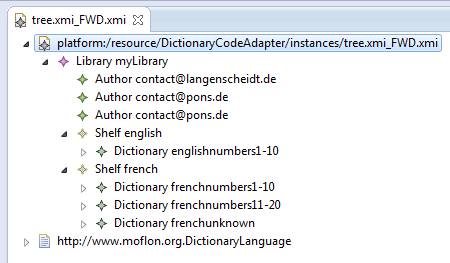
\includegraphics[width=0.7\textwidth]{eclipse_generatedForwardTransformation}
  \caption{completed forward transformation}
  \label{eclipse:generatedFwdTrsfm}
\end{center}
\end{figure}

\item[$\blacktriangleright$] Awesome, it works BEAUTIFULLY! Lets examine the output, \texttt{tree.xmi\_FWD.xmi} a little closer.

\item[$\blacktriangleright$] The transformation decided to take one rule - either create or use existing - based on a random choice. The current set up isn't
dependable. 

\item[$\blacktriangleright$] If you haven't already, read Section 6 from Part IV to learn how eMoflon's integrator feature can help you visualize how this
transformation was completed. Run the integrator on \texttt{corr\_FWD.xmi} until you reach the first (english) author node (do this as proof).

\begin{figure}[htbp]
\begin{center}
  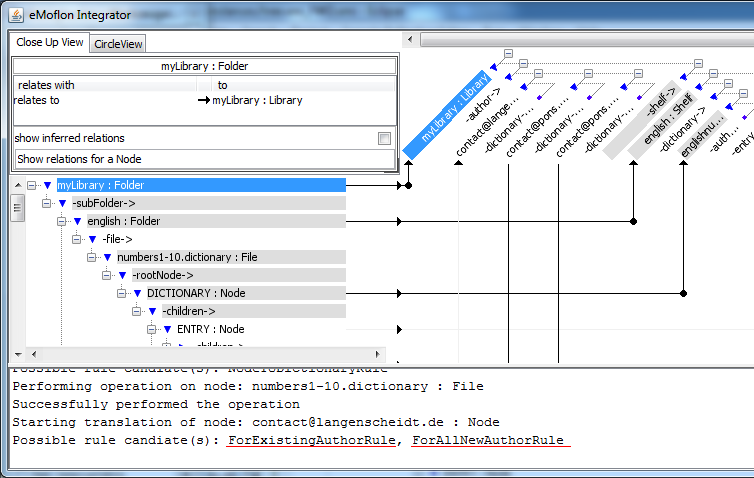
\includegraphics[width=0.7\textwidth]{eclipse_integratorAuthorChoice}
  \caption{completed forward transformation}
  \label{eclipse:generatedFwdTrsfm}
\end{center}
\end{figure}

\item[$\blacktriangleright$] It had two choices and picked on at random. You, dear creator, have two choices on how to refine this. ``I don't care,
\emph{always} make an author'' (duplicates), or no, ``I \emph{never} want there to be two of the same authors for one library.''

\end{itemize}

\begin{description}

\item[option2: Design-time] Create a NAC in \texttt{ForAllNewAuthors}; force it to skip
link1: textual, link 2: visual

\item[option1: Run-time] Create a configuration file for your TGG; INCLUDE HERE

\end{description}